\chapter{A Summer Ball}

The same day during the interview between Madame Danglars and the
procureur, a travelling-carriage entered the Rue du Helder, passed
through the gateway of No. 27, and stopped in the yard. In a moment the
door was opened, and Madame de Morcerf alighted, leaning on her son’s
arm. Albert soon left her, ordered his horses, and having arranged his
toilet, drove to the Champs-Élysées, to the house of Monte Cristo.

The count received him with his habitual smile. It was a strange thing
that no one ever appeared to advance a step in that man’s favor. Those
who would, as it were, force a passage to his heart, found an
impassable barrier. Morcerf, who ran towards him with open arms, was
chilled as he drew near, in spite of the friendly smile, and simply
held out his hand. Monte Cristo shook it coldly, according to his
invariable practice.

“Here I am, dear count.”

“Welcome home again.”

“I arrived an hour since.”

“From Dieppe?”

“No, from Tréport.”

“Indeed?”

“And I have come at once to see you.”

“That is extremely kind of you,” said Monte Cristo with a tone of
perfect indifference.

“And what is the news?”

“You should not ask a stranger, a foreigner, for news.”

“I know it, but in asking for news, I mean, have you done anything for
me?”

“Had you commissioned me?” said Monte Cristo, feigning uneasiness.

“Come, come,” said Albert, “do not assume so much indifference. It is
said, sympathy travels rapidly, and when at Tréport, I felt the
electric shock; you have either been working for me or thinking of me.”

“Possibly,” said Monte Cristo, “I have indeed thought of you, but the
magnetic wire I was guiding acted, indeed, without my knowledge.”

\begin{figure}[ht]
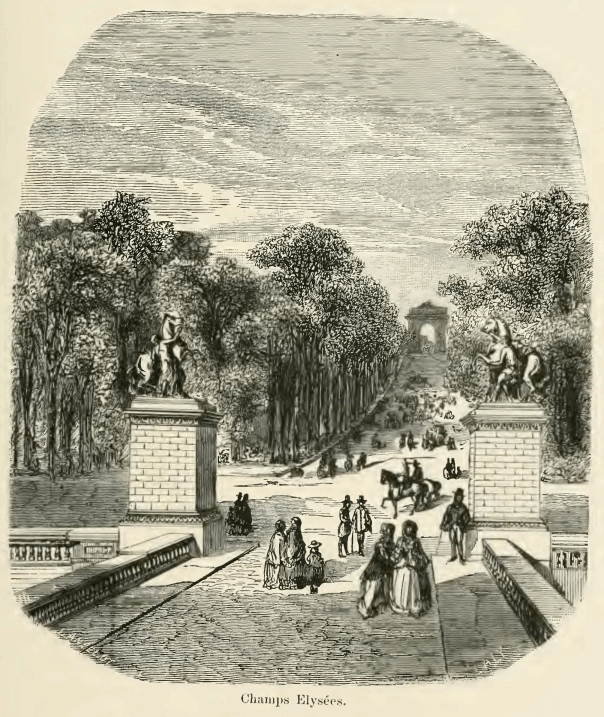
\includegraphics[width=\textwidth]{30277m.jpg}
\end{figure}

“Indeed! Pray tell me how it happened.”

“Willingly. M. Danglars dined with me.”

“I know it; to avoid meeting him, my mother and I left town.”

“But he met here M. Andrea Cavalcanti.”

“Your Italian prince?”

“Not so fast; M. Andrea only calls himself count.”

“Calls himself, do you say?”

“Yes, calls himself.”

“Is he not a count?”

“What can I know of him? He calls himself so. I, of course, give him
the same title, and everyone else does likewise.”

“What a strange man you are! What next? You say M. Danglars dined
here?”

“Yes, with Count Cavalcanti, the marquis his father, Madame Danglars,
M. and Madame de Villefort,—charming people,—M. Debray, Maximilian
Morrel, and M. de Château-Renaud.”

“Did they speak of me?”

“Not a word.”

“So much the worse.”

“Why so? I thought you wished them to forget you?”

“If they did not speak of me, I am sure they thought about me, and I am
in despair.”

“How will that affect you, since Mademoiselle Danglars was not among
the number here who thought of you? Truly, she might have thought of
you at home.”

“I have no fear of that; or, if she did, it was only in the same way in
which I think of her.”

“Touching sympathy! So you hate each other?” said the count.

“Listen,” said Morcerf—“if Mademoiselle Danglars were disposed to take
pity on my supposed martyrdom on her account, and would dispense with
all matrimonial formalities between our two families, I am ready to
agree to the arrangement. In a word, Mademoiselle Danglars would make a
charming mistress—but a wife—\textit{diable!}”

“And this,” said Monte Cristo, “is your opinion of your intended
spouse?”

“Yes; it is rather unkind, I acknowledge, but it is true. But as this
dream cannot be realized, since Mademoiselle Danglars must become my
lawful wife, live perpetually with me, sing to me, compose verses and
music within ten paces of me, and that for my whole life, it frightens
me. One may forsake a mistress, but a wife,—good heavens! There she
must always be; and to marry Mademoiselle Danglars would be awful.”

“You are difficult to please, viscount.”

“Yes, for I often wish for what is impossible.”

“What is that?”

“To find such a wife as my father found.”

Monte Cristo turned pale, and looked at Albert, while playing with some
magnificent pistols.

“Your father was fortunate, then?” said he.

“You know my opinion of my mother, count; look at her,—still beautiful,
witty, more charming than ever. For any other son to have stayed with
his mother for four days at Tréport, it would have been a condescension
or a martyrdom, while I return, more contented, more peaceful—shall I
say more poetic!—than if I had taken Queen Mab or Titania as my
companion.”

\begin{figure}[ht]
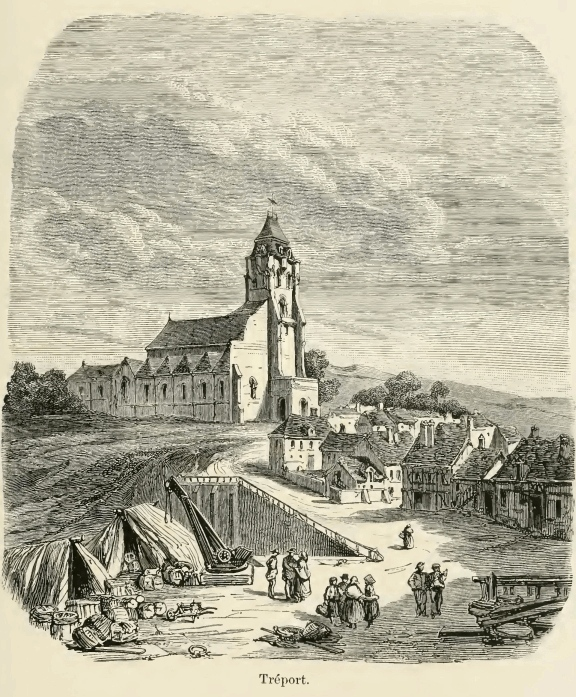
\includegraphics[width=\textwidth]{30279m.jpg}
\end{figure}

“That is an overwhelming demonstration, and you would make everyone vow
to live a single life.”

“Such are my reasons for not liking to marry Mademoiselle Danglars.
Have you ever noticed how much a thing is heightened in value when we
obtain possession of it? The diamond which glittered in the window at
Marlé’s or Fossin’s shines with more splendor when it is our own; but
if we are compelled to acknowledge the superiority of another, and
still must retain the one that is inferior, do you not know what we
have to endure?”

“Worldling,” murmured the count.

“Thus I shall rejoice when Mademoiselle Eugénie perceives I am but a
pitiful atom, with scarcely as many hundred thousand francs as she has
millions.” Monte Cristo smiled. “One plan occurred to me,” continued
Albert; “Franz likes all that is eccentric; I tried to make him fall in
love with Mademoiselle Danglars; but in spite of four letters, written
in the most alluring style, he invariably answered: ‘My eccentricity
may be great, but it will not make me break my promise.’”

“That is what I call devoted friendship, to recommend to another one
whom you would not marry yourself.” Albert smiled.

“Apropos,” continued he, “Franz is coming soon, but it will not
interest you; you dislike him, I think?”

“I?” said Monte Cristo; “my dear viscount, how have you discovered that
I did not like M. Franz! I like everyone.”

“And you include me in the expression everyone—many thanks!”

“Let us not mistake,” said Monte Cristo; “I love everyone as God
commands us to love our neighbor, as Christians; but I thoroughly hate
but a few. Let us return to M. Franz d’Épinay. Did you say he was
coming?”

“Yes; summoned by M. de Villefort, who is apparently as anxious to get
Mademoiselle Valentine married as M. Danglars is to see Mademoiselle
Eugénie settled. It must be a very irksome office to be the father of a
grown-up daughter; it seems to make one feverish, and to raise one’s
pulse to ninety beats a minute until the deed is done.”

“But M. d’Épinay, unlike you, bears his misfortune patiently.”

“Still more, he talks seriously about the matter, puts on a white tie,
and speaks of his family. He entertains a very high opinion of M. and
Madame de Villefort.”

“Which they deserve, do they not?”

“I believe they do. M. de Villefort has always passed for a severe but
a just man.”

“There is, then, one,” said Monte Cristo, “whom you do not condemn like
poor Danglars?”

“Because I am not compelled to marry his daughter perhaps,” replied
Albert, laughing.

“Indeed, my dear sir,” said Monte Cristo, “you are revoltingly
foppish.”

“I foppish? how do you mean?”

“Yes; pray take a cigar, and cease to defend yourself, and to struggle
to escape marrying Mademoiselle Danglars. Let things take their course;
perhaps you may not have to retract.”

“Bah!” said Albert, staring.

“Doubtless, my dear viscount, you will not be taken by force; and
seriously, do you wish to break off your engagement?”

“I would give a hundred thousand francs to be able to do so.”

“Then make yourself quite easy. M. Danglars would give double that sum
to attain the same end.”

“Am I, indeed, so happy?” said Albert, who still could not prevent an
almost imperceptible cloud passing across his brow. “But, my dear
count, has M. Danglars any reason?”

“Ah! there is your proud and selfish nature. You would expose the
self-love of another with a hatchet, but you shrink if your own is
attacked with a needle.”

“But yet, M. Danglars appeared——”

“Delighted with you, was he not? Well, he is a man of bad taste, and is
still more enchanted with another. I know not whom; look and judge for
yourself.”

“Thank you, I understand. But my mother—no, not my mother; I mistake—my
father intends giving a ball.”

“A ball at this season?”

“Summer balls are fashionable.”

“If they were not, the countess has only to wish it, and they would
become so.”

“You are right; You know they are select affairs; those who remain in
Paris in July must be true Parisians. Will you take charge of our
invitation to Messieurs Cavalcanti?”

“When will it take place?”

“On Saturday.”

“M. Cavalcanti’s father will be gone.”

“But the son will be here; will you invite young M. Cavalcanti?”

“I do not know him, viscount.”

“You do not know him?”

“No, I never saw him until a few days since, and am not responsible for
him.”

“But you receive him at your house?”

“That is another thing: he was recommended to me by a good abbé, who
may be deceived. Give him a direct invitation, but do not ask me to
present him. If he were afterwards to marry Mademoiselle Danglars, you
would accuse me of intrigue, and would be challenging me,—besides, I
may not be there myself.”

“Where?”

“At your ball.”

“Why should you not be there?”

“Because you have not yet invited me.”

“But I come expressly for that purpose.”

“You are very kind, but I may be prevented.”

“If I tell you one thing, you will be so amiable as to set aside all
impediments.”

“Tell me what it is.”

“My mother begs you to come.”

“The Comtesse de Morcerf?” said Monte Cristo, starting.

“Ah, count,” said Albert, “I assure you Madame de Morcerf speaks freely
to me, and if you have not felt those sympathetic fibres of which I
spoke just now thrill within you, you must be entirely devoid of them,
for during the last four days we have spoken of no one else.”

“You have talked of me?”

“Yes, that is the penalty of being a living puzzle!”

“Then I am also a puzzle to your mother? I should have thought her too
reasonable to be led by imagination.”

“A problem, my dear count, for everyone—for my mother as well as
others; much studied, but not solved, you still remain an enigma, do
not fear. My mother is only astonished that you remain so long
unsolved. I believe, while the Countess G—— takes you for Lord Ruthven,
my mother imagines you to be Cagliostro or the Count Saint-Germain. The
first opportunity you have, confirm her in her opinion; it will be easy
for you, as you have the philosophy of the one and the wit of the
other.”

“I thank you for the warning,” said the count; “I shall endeavor to be
prepared for all suppositions.”

“You will, then, come on Saturday?”

“Yes, since Madame de Morcerf invites me.”

“You are very kind.”

“Will M. Danglars be there?”

“He has already been invited by my father. We shall try to persuade the
great d’Aguesseau,\footnote[11]{Magistrate and orator of great
eloquence—chancellor of France under Louis XV.} M. de Villefort, to come,
but have not much hope of seeing him.”

“‘Never despair of anything,’ says the proverb.”

“Do you dance, count?”

“I dance?”

“Yes, you; it would not be astonishing.”

“That is very well before one is over forty. No, I do not dance, but I
like to see others do so. Does Madame de Morcerf dance?”

“Never; you can talk to her, she so delights in your conversation.”

“Indeed?”

\begin{figure}[ht]
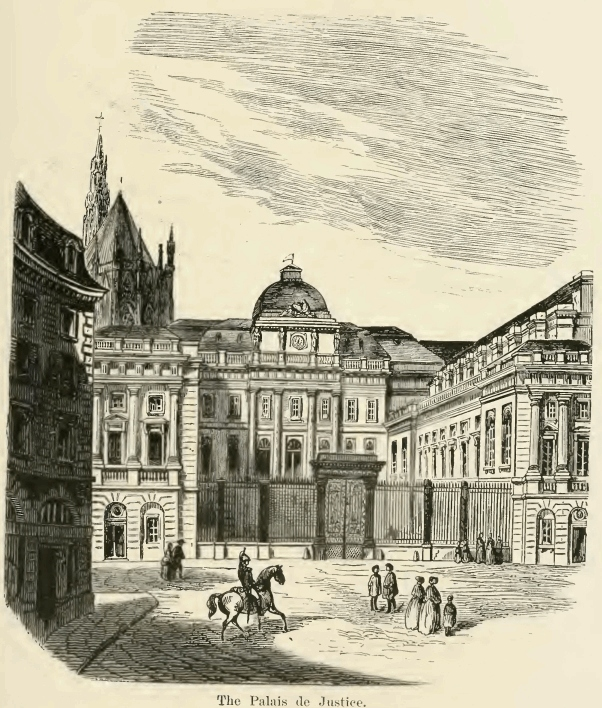
\includegraphics[width=\textwidth]{30283m.jpg}
\end{figure}

“Yes, truly; and I assure you. You are the only man of whom I have
heard her speak with interest.” Albert rose and took his hat; the count
conducted him to the door.

“I have one thing to reproach myself with,” said he, stopping Albert on
the steps. “What is it?”

“I have spoken to you indiscreetly about Danglars.”

“On the contrary, speak to me always in the same strain about him.”

“I am glad to be reassured on that point. Apropos, when do you aspect
M. d’Épinay?”

“Five or six days hence at the latest.”

“And when is he to be married?”

“Immediately on the arrival of M. and Madame de Saint-Méran.”

“Bring him to see me. Although you say I do not like him, I assure you
I shall be happy to see him.”

“I will obey your orders, my lord.”

“Good-bye.”

“Until Saturday, when I may expect you, may I not?”

“Yes, I promised you.” The Count watched Albert, waving his hand to
him. When he had mounted his phaeton, Monte Cristo turned, and seeing
Bertuccio, “What news?” said he.

“She went to the Palais,” replied the steward.

“Did she stay long there?”

“An hour and a half.”

“Did she return home?”

“Directly.”

“Well, my dear Bertuccio,” said the count, “I now advise you to go in
quest of the little estate I spoke to you of in Normandy.”

Bertuccio bowed, and as his wishes were in perfect harmony with the
order he had received, he started the same evening.
